\documentclass[a4paper,twocolumn]{article}

\usepackage{graphicx}
\usepackage[small]{caption}

\begin{document}

\title{Automatic Structural Inference of Binary Protocols}
\author{Fredrik Appelros \and Carl Ekerot}
\maketitle

\begin{abstract}
Communication protocols are the foundation of everyday networking tasks but
they are not always open in terms of available documentation. For reasons of
interoperability or the collection of statistics some protocols need to be
reverse engineered. This article presents a method based on density-based
clustering and byte distribution classification for automatically inferring the
structure of a protocol from a packet dump. We evaluate the precision of the
method for finding different packet types and for finding fields globally
across all packets.
\end{abstract}

\section{Introduction}
The languages computers use when communicating are defined in network protocols.
Some of these protocols, like HTTP, are text-based but a large portion of them
are binary. Text-based protocols use messages that are easy for humans to
understand as they can simply be read while binary ones are much harder to
interpret. Binary protocols consist of a large chunk of binary data with no
clear distinction between the different parts. However, each protocol usually
has a documentation that explains how to interpret this data; a definition of
the different fields that the data chunks are made up of. A field is a set of
bits that represent some kind of information. It can be a flag, a number, a
string or just raw data.

Unfortunately, this documentation is not always available. The protocol might
be proprietary or simply undocumented, making it hard for third parties to use.
For interoperability or quality of service reasons the demand to understand
these protocols still exists. This is where protocol reverse engineering steps
in. Protocol reverse engineering is the art of deducing the syntax and
semantics of a protocol by analyzing its communication.

\section{Method}
The approach we used is based on analysis of packet dumps, i.e. a collection
of captured messages. The first step was to find the different message types.
After this was done we focused on finding different types of fields; both
common for all types and unique fields within types. Lastly, we also
constructed a state diagram for the protocol to get an overview of the
transitions between different message types.

\subsection{Type inference}
The first part was done with the help of a density-based clustering algorithm
called \emph{OPTICS}. What this step does is group similar messages together into
\emph{clusters}. The similarity of the messages are defined as the euclidean
distance between them in a feature-space. For our features we chose the
observed probability of the current byte value occurring at the current
position for each position in the message. This works fairly well but becomes
cumbersome as the feature-space will be $n$-dimensional where $n$ is the size
of the largest message. To circumvent this we apply
\emph{principal component analysis} (PCA) on all our features to reduce the
dimensionality of the problem.

This yields a fairly good result but it can still be improved upon. We further
assume that this initial clustering is mostly homogeneous, i.e. most clusters
only contain messages of a single type. We also assume that there is some set
of bytes in the message that indicates what type it is. We call these bytes
\emph{type distinguishers}. We then refine our clustering by finding the bytes
that are most likely to be type distinguishers and grouping messages together
depending on the values of these bytes. The most likely candidates are found by
measuring how high the \emph{completeness} for the clusters becomes if they are
grouped together by the value of that specific byte. Completeness is a metric
that describes how spread out the different message types are. If all messages
of each specific type is located in a single cluster the completeness becomes
one while on the other hand if all messages are located in different clusters
it becomes zero. In most clusterings the completeness value falls somewhere
in between zero and one. With the type distinguishers and, therefore, the
message types found we move on to the next step; finding the fields.

\subsection{Field inference}
When inferring the fields we start by defining a set of field types that we
deem identifiable, e.g. length fields, flags and constants. We then go through
all possible aligned field positions of different lengths and try to match them
to one of these types. This is done for different scopes of our packet dump in
order to find fields present in all messages as well as fields only present in
certain types.

For some of the more basic types, like flags and constants, it is sufficient to
look at the distribution of byte values for each byte of the potential field in
order to determine the field type. The distribution are constructed from all
the messages in the current scope. For more complex types a deeper analysis is
needed. A good example is length fields for which we do a robust form of linear
regression to see if we can find some linear dependency between the value in
the field and the lengths of the messages.

Once we have all the possible field types for all possible aligned field
positions we merge them together into a unified definition. The merging works
on a set of precedences for the types in order to remove overlapping fields.

\begin{figure}[h]
    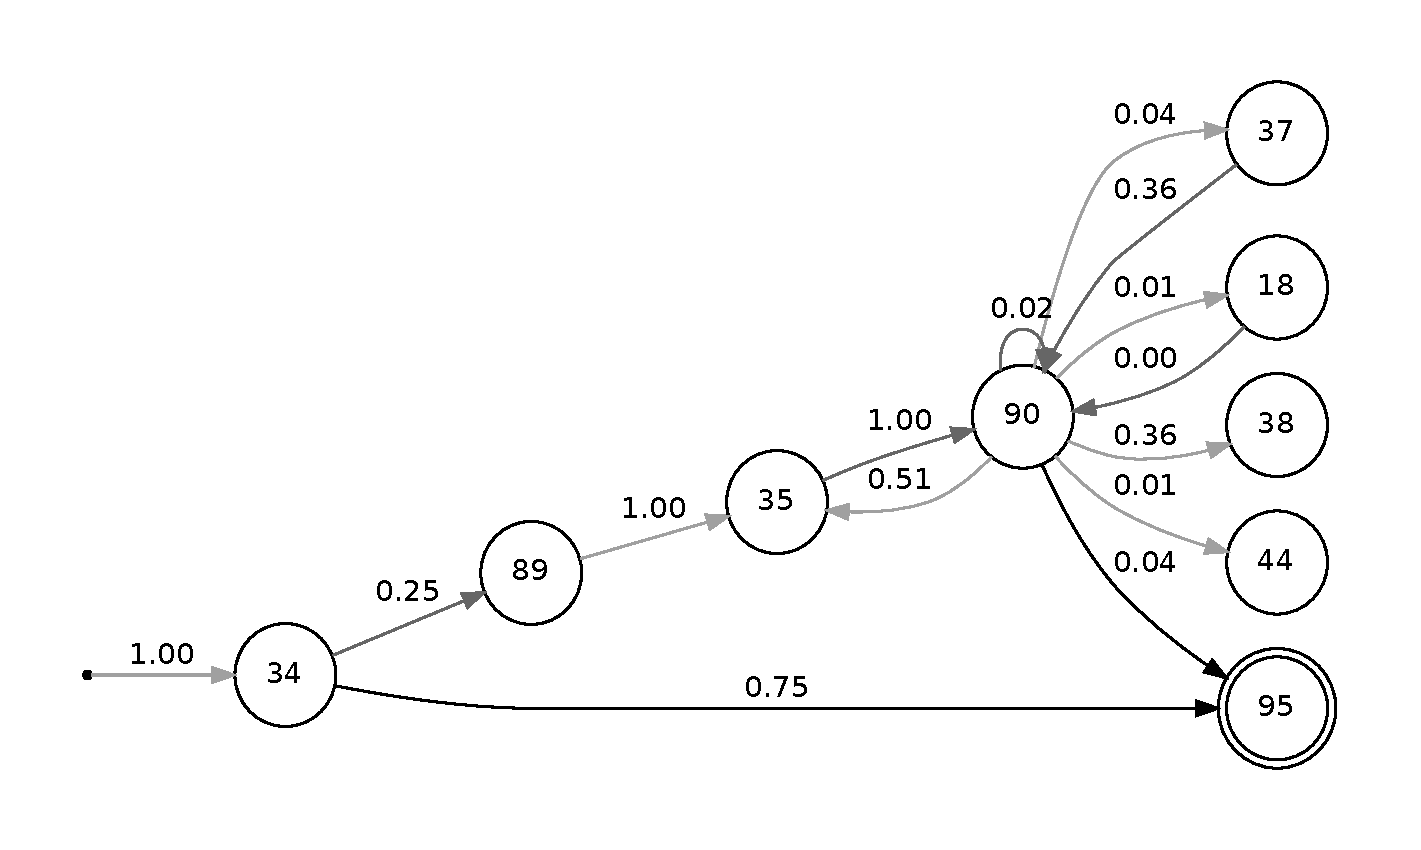
\includegraphics[width=\linewidth]{img/smbstate}
    \caption{State diagram for the first five states of the SMB protocol. A
        handshaking procedure is clearly visible in the first three states.}
    \label{fig:smbstate}
\end{figure}

\subsection{State inference}
For our state diagram we only want a simple overview of the first few states
of the protocol. Because of this we have a parameter that limits the diagram to
a number of transitions from the start state. The diagram itself is constructed
by building a pair of transition matrices from the connections in the packet
dump. Each inferred message type is considered a state and sequential messages
are seen as state transitions. Using these matrices it is trivial to produce a
state diagram for the protocol. An example of such a diagram is seen in
figure~\ref{fig:smbstate}.

\section{Results}
We have measured the performance for each stage of our method on five
different datasets generated from five different protocols. For the two
clustering passes we measured completeness, homogenity and \emph{V-measure}.
V-measure is a metric that reflects how good both the homogenity and the
completeness are. 

After the OPTICS clustering pass, we found that the homogenity was generally
high while completeness was low. This means that the clusters mainly
consisted of a single true message type, but that messages from each true
message type was spread out over more than one cluster. As a consequence the
V-measure was pretty low as well.

The refining pass successfully found some or all of the type distinguishers
in four of the five datasets. For the datasets where all type distinguishers
were found our metrics resulted in a next to perfect score. In one dataset
only one of its two type distinguishers was found which resulted in perfect
completeness but a mediocre homogenity. In another dataset where no
type distinguishers were found the completeness and V-measure scores were as
low as possible. This was expected since the dataset only contained messages
from a single type.

When measuring the field inference performance we introduced our own metric.
The metric we used was the ratio of bits correctly inferred with respect to
each protocol specification. Our method yielded up to 41.7\% correctly
inferred bits. In worst case 0\% of the bits were correctly inferred.
Using this metric, a result of 100\% correctly inferred bits is unrealistic
since some field values never occur or are in practice only a single value
although the protocol specification labels it as e.g. a flag.

\section{Discussion}
Our method for finding message types works very well for datasets where more
than one message type is present. From our evaluation of our method we have
learned that a diverse dataset is crucial for a good analysis to be possible.

We have observed that our field inference often finds field types that reflect
how the field is actually used in the protocol. Our field inference reveals
information on the type of data that is stored in a field, and gives an
indication of the boundaries of the field. We believe that this method could
be improved further, and that it could be extended to more field types such
as timestamps.
\end{document}

